Things to note: KiCAD produces gerber files in 274X format, so an aperture list file isn't needed.  Use 8 characters for the file names.  The drill map needs to be precision 2:4 with trailing zeros suppressed.

To generate the gerber and drill files, in Pcbnew, go to file-->plot, see Figure~\ref{fig:plotdialog1}.  Notice that the copper layers, silkscreen, soldermask, and PCB\_Edges layers are selected; that "Exclude PCB Edge layer from other layers" is selected; and that "Use auxiliary axis as origin" is selected.  A folder in the project directory called "gerber" keeps the plotted files organized.  Press "Plot" to generate the files.

\begin{figure}[H]
	\centering 
		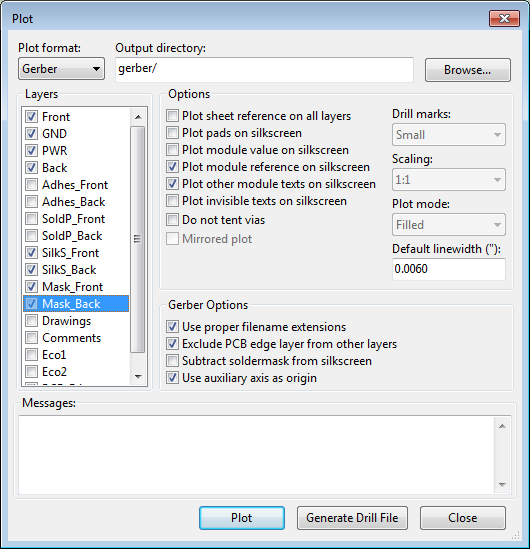
\includegraphics{./figures/plotdialog1} 
	\caption{Pcbnew plot dialog\label{fig:plotdialog1}}
\end{figure}

Advanced Circuits prefers the edge outline of the PCB to be on the silkscreen layer rather than in a separate file.  As set up in Figure~\ref{fig:plotdialog1}, the edges are only in the separate file.  To get the edges on the front silkscreen, see  Figure~\ref{fig:plotdialog2}.  Notice that only the front silkscreen layer is selected and this time "Exclude PCB Edge layer from other layers" is not selected. Press "Plot" to generate the new front silkscreen with the PCB edges.

\begin{figure}[H]
	\centering 
		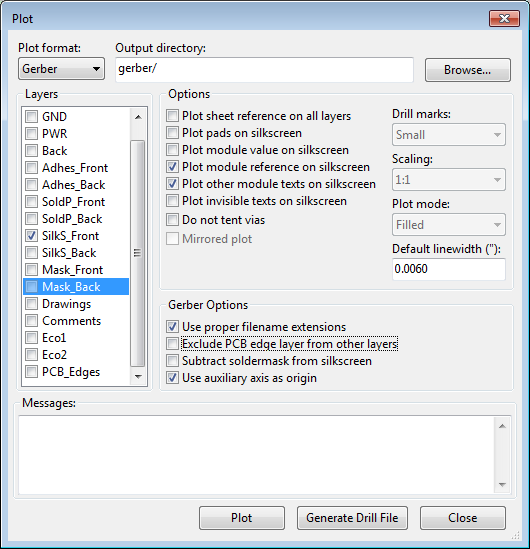
\includegraphics{./figures/plotdialog2} 
	\caption{Pcbnew plot dialog\label{fig:plotdialog2}}
\end{figure}

To generate the drill file, while in file-->plot, press the "Generate Drill File" button.  See  Figure~\ref{fig:drilldialog}.  Notice the Inches, Suppress trailing zeros, 2:4 precision, Drill Map (gerber), and the auxiliary axis that should have been added to the layout are selected (the auxiliary axis was also selected in Figure~\ref{fig:plotdialog1}).  It is necessary to have set the auxiliary axis to a corner of the PCB outline in the main drawing window.  The Drill Map (gerber) selection will produce the additional "fabrication print showing printed circuit board outline with drill pattern and sizes in gerber format."

\begin{figure}[H]
	\centering 
		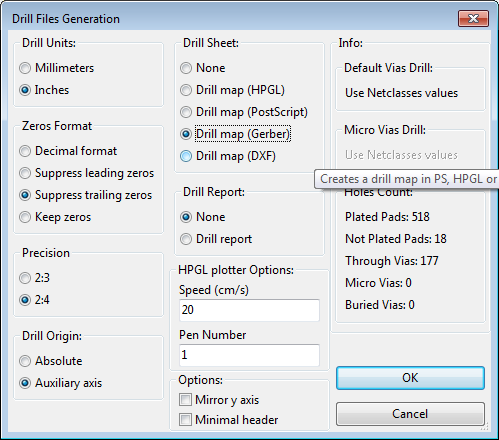
\includegraphics{./figures/drilldialog} 
	\caption{Pcbnew drill dialog\label{fig:drilldialog}}
\end{figure}

When going through the FreeDFM:

You will have to select what each file is.  The program recognizes most files, except for the PCB\_Edges which you want to set as "Drawing/Other" in the drop down box and the GND and PWR layers are "Inner Copper" in the dropdown and another drop down will show up in which you tell it that the files are "Positive" (the filled in areas should have copper as opposed to negative in which the filled in areas are not copper) and GND is layer "2" (or "3") while PWR is layer "3" (or "2") (if th  The .drl file is the Excellion dril file while the .pho file is the fabrication print with drill pattern and sizes in gerber format that should be "Drawing/Other."  %See Figure~\ref{fig:freedfm}

%\begin{landscape}
%\begin{figure}[h]
%	\centering 
%	\begin{singlespace}
%	\begin{subfigure}[b]{0.45\textwidth}
%		\centering 
%		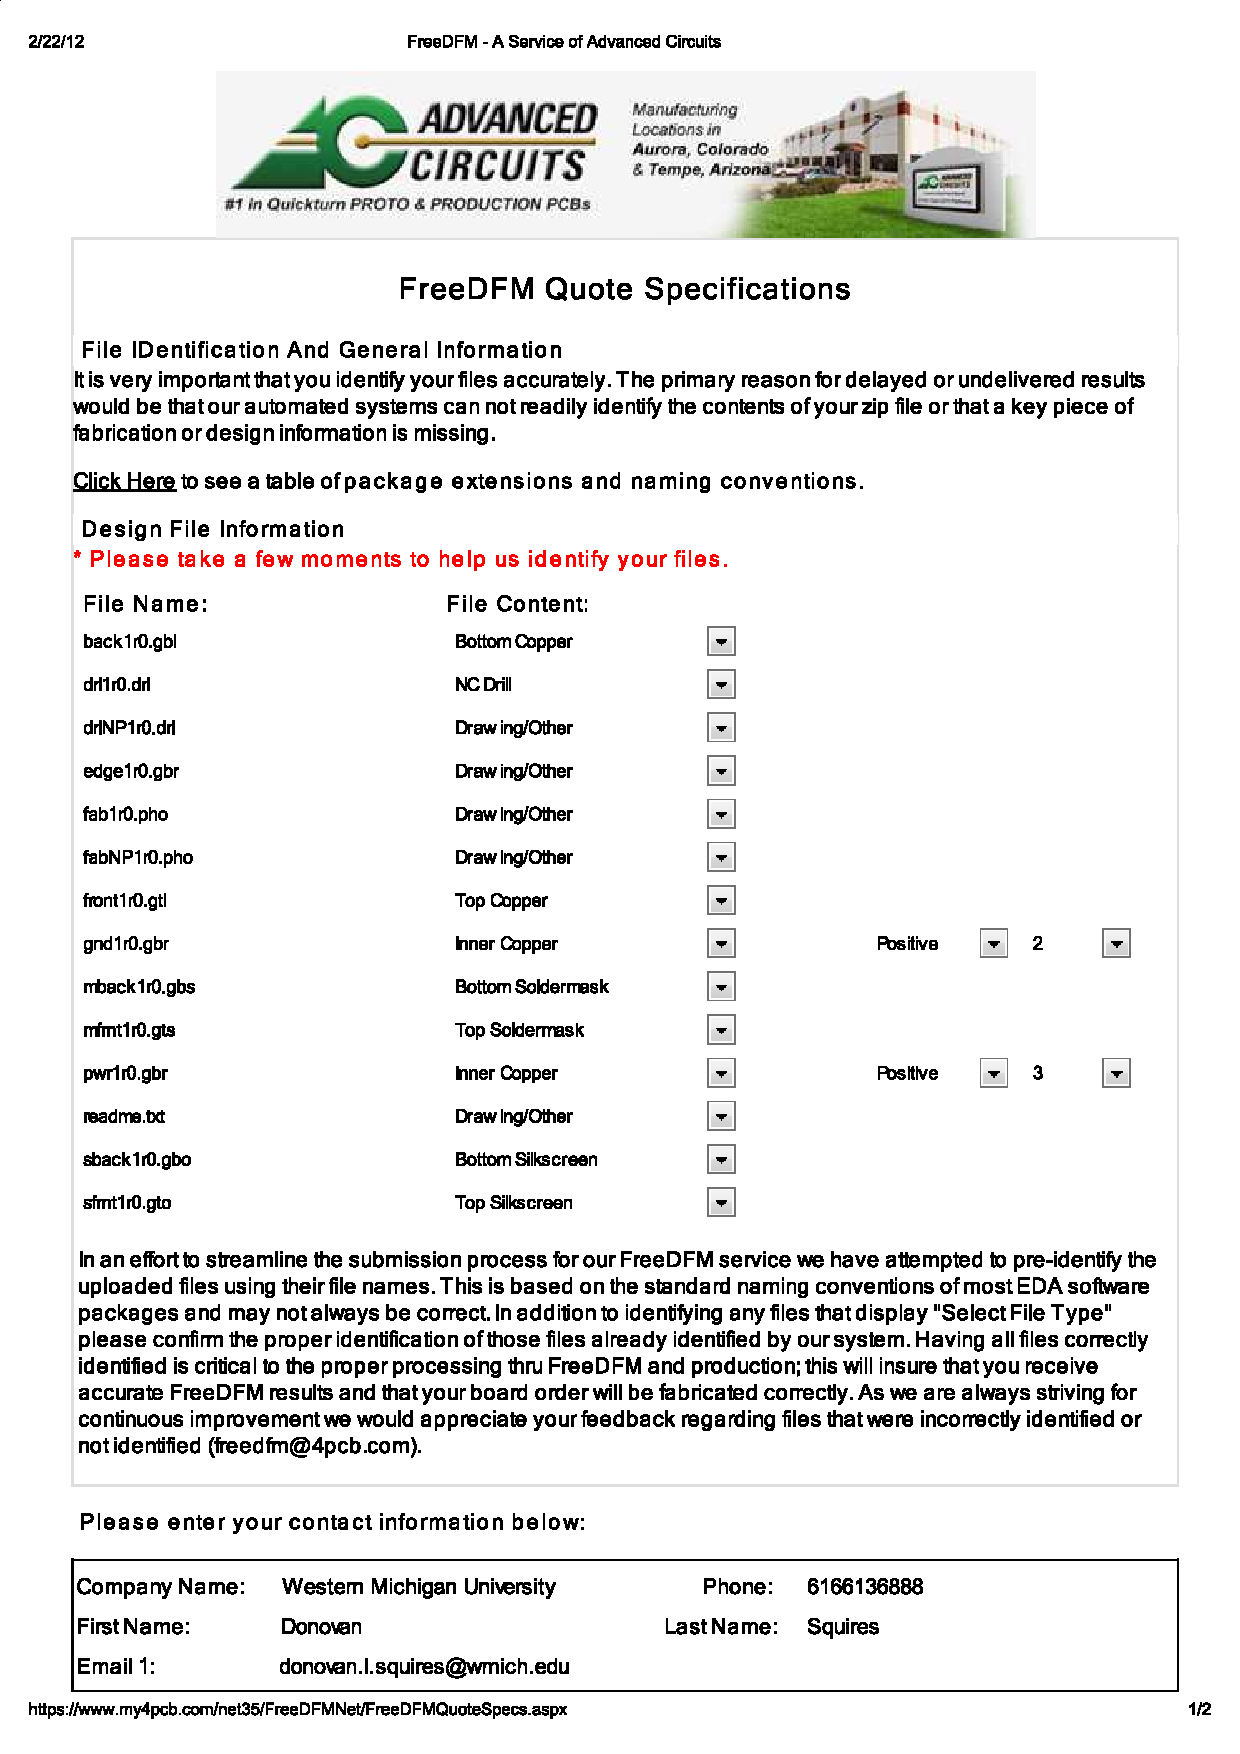
\includegraphics[page=1,height=0.9\textheight]{./figures/FreeDFMupload_120222}
%	\caption{Power plane\label{fig:freedfma}}
%	\end{subfigure}
%	~
%	\begin{subfigure}[b]{0.45\textwidth}
%		\centering 
%		\includegraphics[page=2,height=0.9\textheight]{./figures/FreeDFMupload_120222}
%	\caption{Ground plane\label{fig:freedfmb}}
%	\end{subfigure}
%	\caption{Close clearances on power and ground planes\label{fig:freedfm}}
%	\end{singlespace}
%\end{figure}
%\end{landscape}

When you are ready to place your order:

\begin{enumerate}
	\item Add a README.txt with this information:
	\begin{enumerate}
		\item List of every file name with a brief description as to what it is.
		\item List all non-gerber specs for this job.
		\item Your contact information (include evening phone if you like).
	\end{enumerate}
	\item Change all of the file names to 8 characters + the 3 character extension
	\item Remember that if you place orders later, you will want to have a different zip file name.
\end{enumerate}